\documentclass[11pt]{article}

\newcommand{\squishlist}{
   \begin{list}{$\bullet$}
    { \setlength{\itemsep}{0pt}      \setlength{\parsep}{3pt}
      \setlength{\topsep}{3pt}       \setlength{\partopsep}{0pt}
      \setlength{\leftmargin}{1.5em} \setlength{\labelwidth}{1em}
      \setlength{\labelsep}{0.5em} } }

\newcommand{\squishend}{
    \end{list}  }

\usepackage{times}
\usepackage{mathptm}
\usepackage{fullpage}
\usepackage{graphicx}

\begin{document}

\begin{center}
{\bf{Regis University -- Physics 305A -- Fall 2019}} \\
{\bf{Lab 11: Moments of Inertia}} \\
\end{center}

In this lab, you will measure the moments of inertia of a number of different
objects, comparing your experimental results with calculations based on
the geometry of the objects.  Just like last week, you will need to 
think through the details of how to do the experiment.

\bigskip

\begin{enumerate}
\item Connect the rotational motion sensor to the computer through 
the DIG/SONIC 1 port on the Vernier LabPro interface, and run the 
Logger Pro software.  This is one of the few sensor types that cannot be 
automatically detected and configured by the software; you will need to 
select it using the dialog box that appears when you choose the menu option
``Experiment $\rightarrow$ Set Up Sensors $\rightarrow$ LabPro: 1.''  
In that dialog box, use the pop-up menu under DIG/SONIC 1 and 
select ``Choose Sensor... $\rightarrow$ Rotary Motion.''
This sensor measures the angle through which the pulley on top is turned.  
Collect some practice runs, turning the pulley by hand, to convince yourself 
that you understand what the computer is displaying.
\item Mount the rotational motion sensor on a support rod and clamp it to 
the edge of your table.  Tie a thread onto one of the small holes in the 
pulley on top of the sensor, and route the thread
over the clamp-on ``Super Pulley'' and towards the floor.  This configuration 
is illustrated in the left photograph below.  Tie a hanger with a known mass 
to the other end of the thread.
\begin{center}
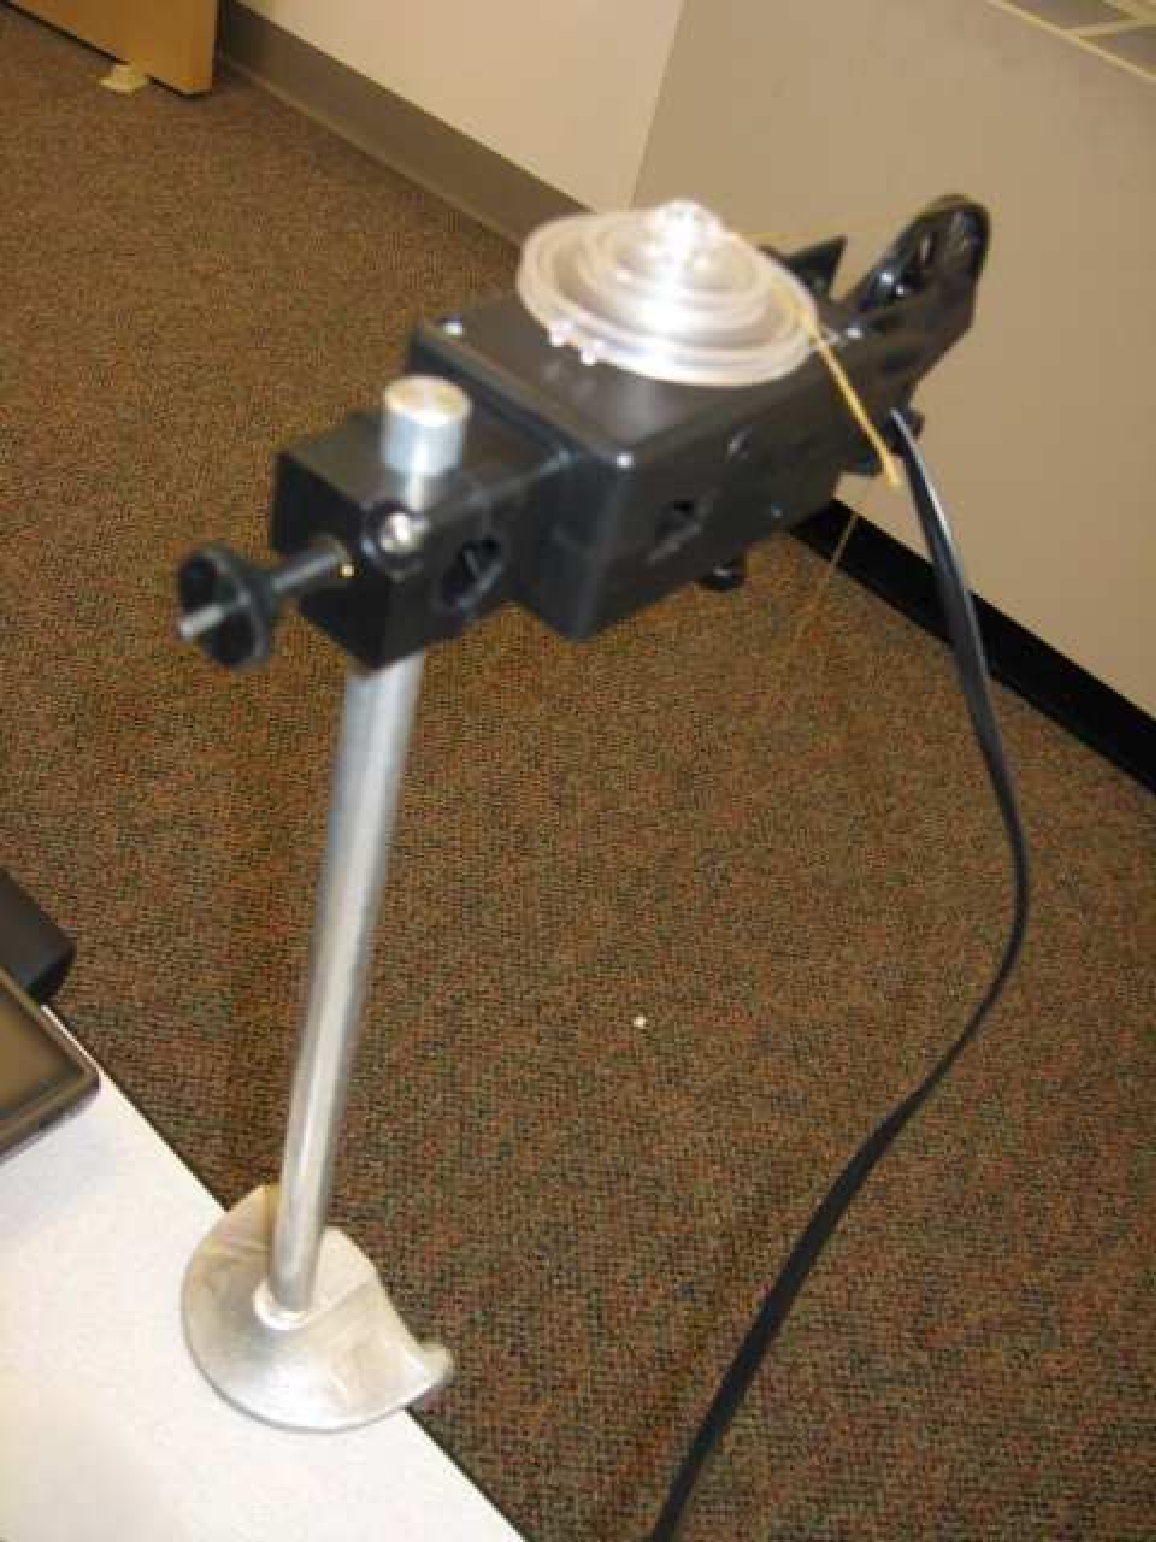
\includegraphics[height=0.30\textheight]{rot1.pdf}
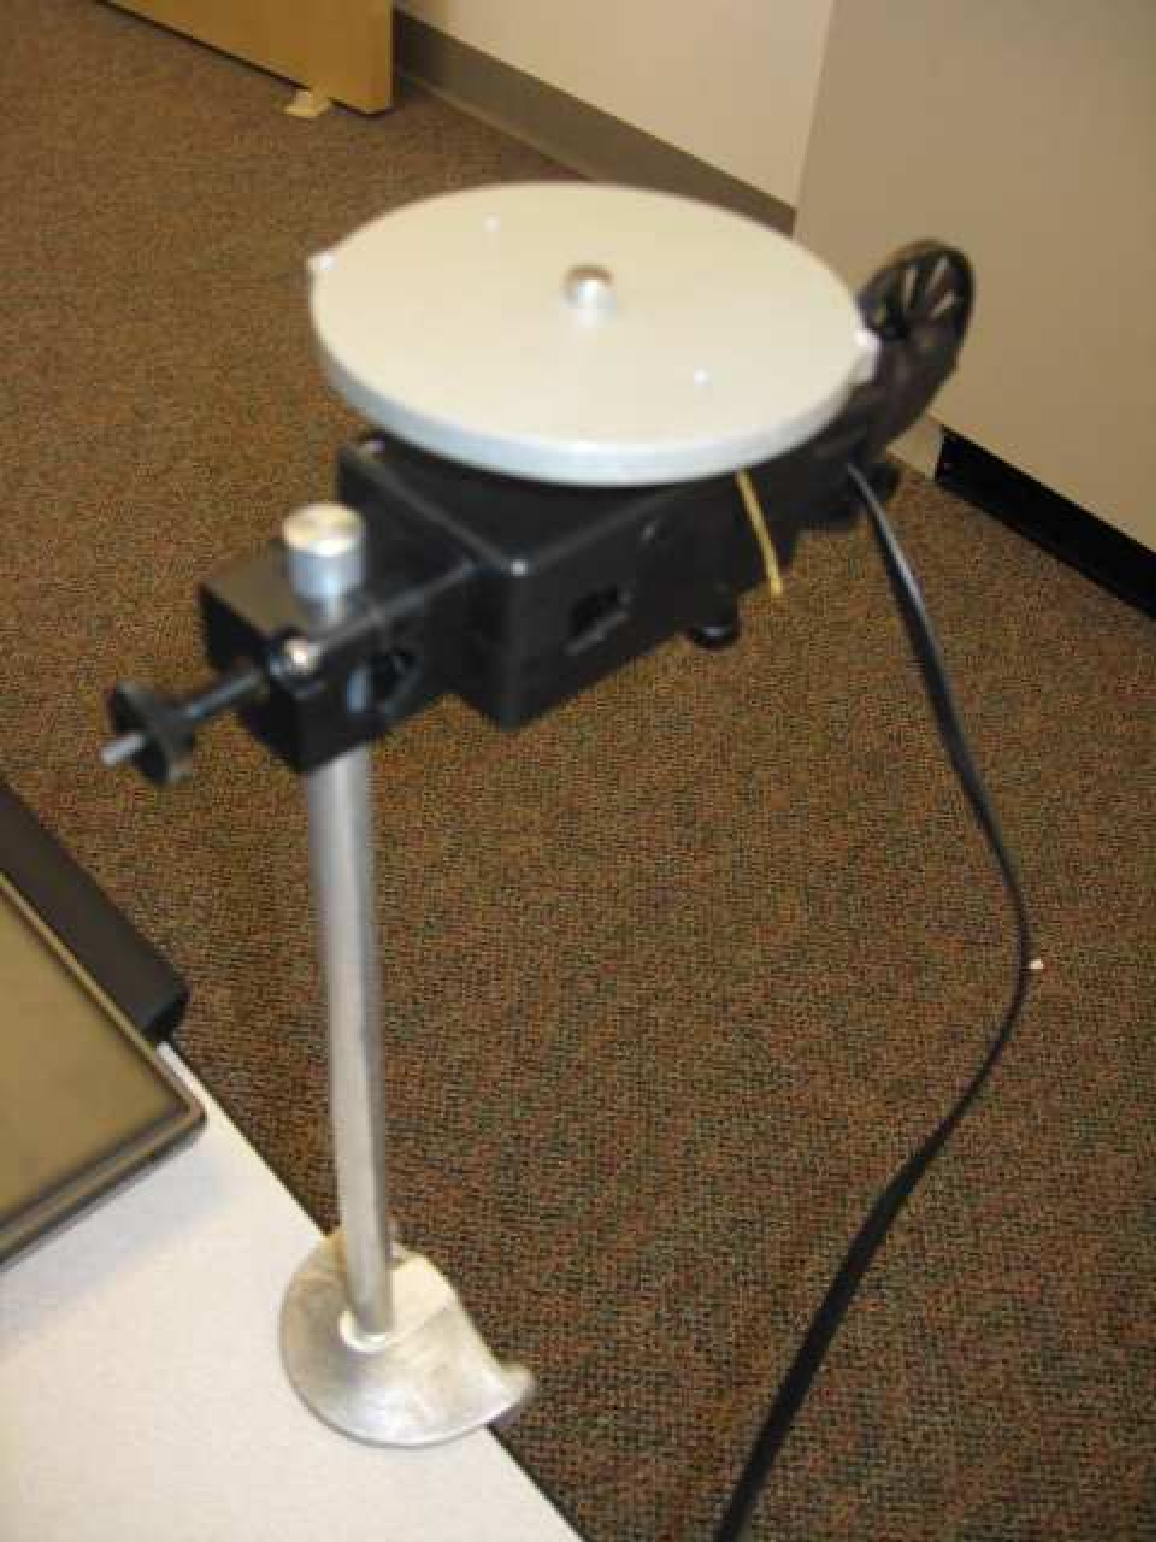
\includegraphics[height=0.30\textheight]{rot2.pdf}
\end{center}
\item Wind the thread up around the top pulley.  While collecting data with
the computer, allow the mass hanger to drop through a known distance to the 
floor.  This will convert the gravitational potential energy primarily 
into (a) rotational kinetic energy of the spinning pulley (and the gear system 
to which it is attached), and (b) translational kinetic energy of the mass 
hanger.  
\item The computer will read out for you the total angle $\theta$ through
which the pulley has been turned (units of radians), as well as the angular
speed $\omega = \frac{d \theta}{d t}$ (units of radians per second).  How can
you use this information to measure the linear speed at which the mass hanger
fell?  (What other measurements will you neeed to make?)  
You will need to know this speed in order to account for its translational 
kinetic energy.
\item Based on your data, and using the law of conservation of energy,  
determine the moment of inertia of the rotational motion sensor and the
pulley attached to it.  
\item Mount the aluminum disk on top of the pulley, as shown in the 
photograph on the right above.  Use the same technique to experimentally
determine its moment of inertia.  (Remember to 
subtract the moment of inertia of the pulley system.)
\item Measure the mass and the diameter of the aluminum disk, and 
{\em{calculate}} its moment of inertia (via $I = \alpha M R^2$).  Compare with your experimental result.
\item Place the steel ring on top of the aluminum disk; the bumps on the
bottom of the ring fit into the holes on the disk to secure it.  Find the
moment of inertia of the steel ring.
\item Measure the mass and diameter of the steel ring, and {\em{calculate}} 
its moment of inertia.  Compare with your experimental result.
\end{enumerate}

\noindent In summary, you should measure the moments of inertia of:
\begin{itemize}
\item The ``bare'' pulley system.
\item The aluminum disk.
\item The steel ring.
\end{itemize}
...and compare your experimental measurements against calculations based on 
their geometries.  If you have the time and interest, you can also experiment 
with a light rod to which sliding masses may be attached.


\end{document}
